\documentclass[11pt, a4paper]{article}

\usepackage{graphicx}
\usepackage[english]{babel}
\usepackage[utf8x]{inputenc}
\usepackage{amsmath}
\usepackage[a4paper,top=3cm,bottom=2cm,left=2cm,right=2cm,marginparwidth=1.75cm]{geometry}
\usepackage{amssymb}
\usepackage{subfig}

\graphicspath{ {./images} }
\newcommand*{\qed}{\hfill\ensuremath{\quad\square}}%
\newcommand*{\rad}{\ensuremath{\,\text{rad}}}
\newcommand*{\R}{\ensuremath{\mathbb{R}}}

\makeatletter
\renewcommand*\env@matrix[1][*\c@MaxMatrixCols c]{%
  \hskip -\arraycolsep
  \let\@ifnextchar\new@ifnextchar
  \array{#1}}
\makeatother

\newtheorem{theorem}{Theorem}

%------------------------------------------------
%Templates for images and figures
% \begin{figure}[h]
%   \centering
%   \subfloat[caption 1]{{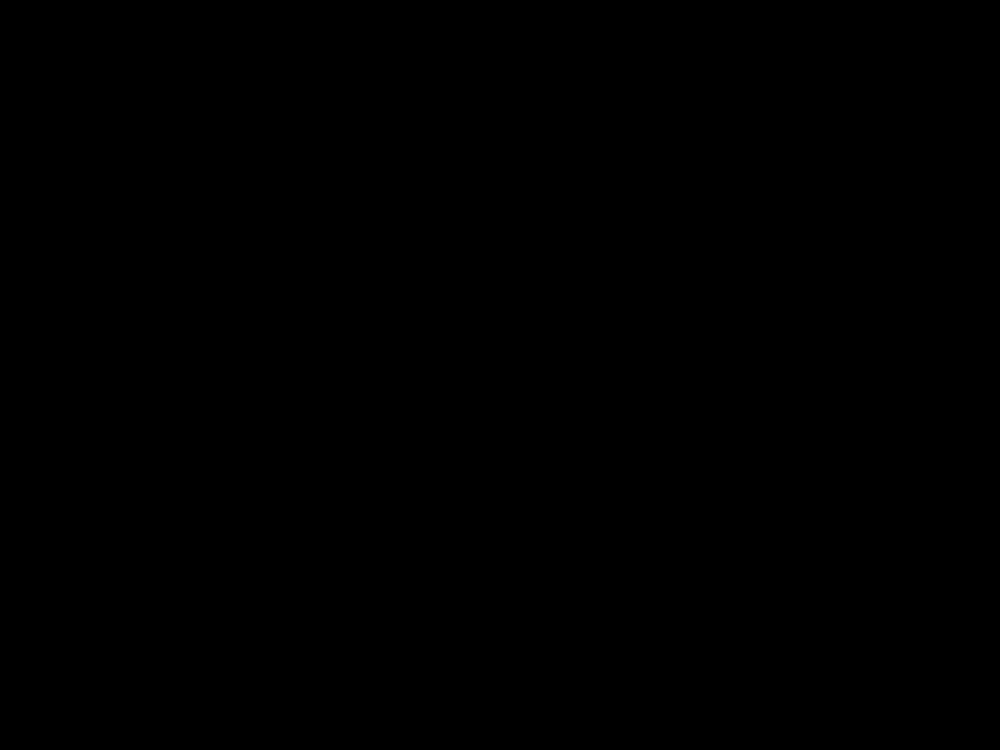
\includegraphics[width=30mm]{images/placeholder.png}}}%
%   \qquad
%   \subfloat[caption 2]{{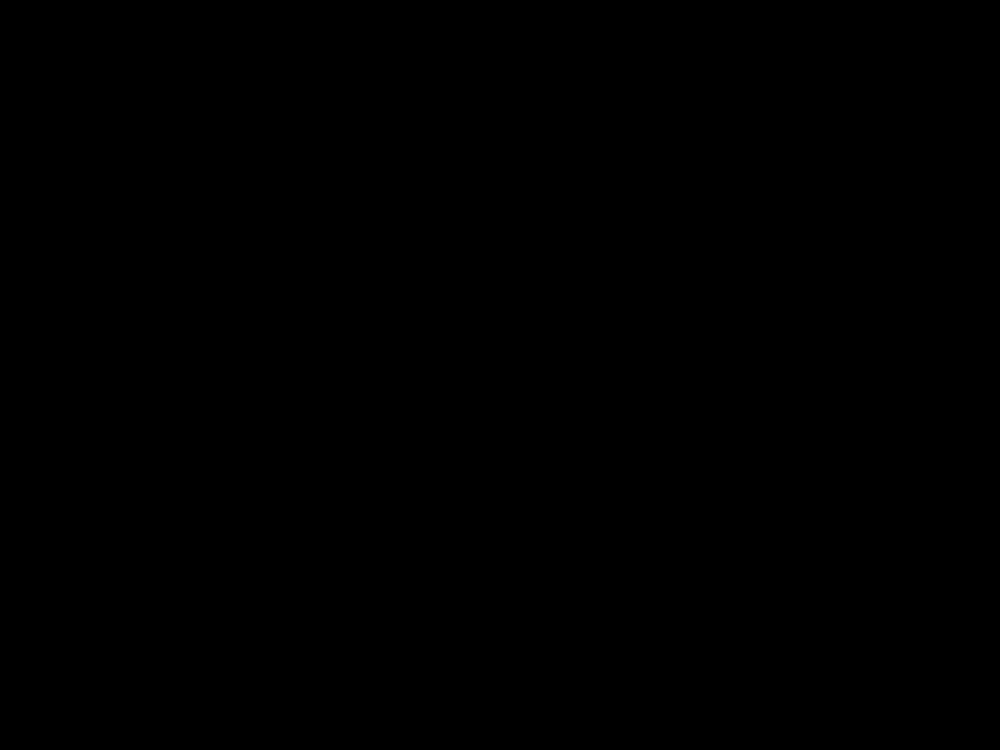
\includegraphics[width=30mm]{images/placeholder.png}}}%
%   \caption{Description}
% \end{figure}

% \begin{figure}[h]
%   \centerline{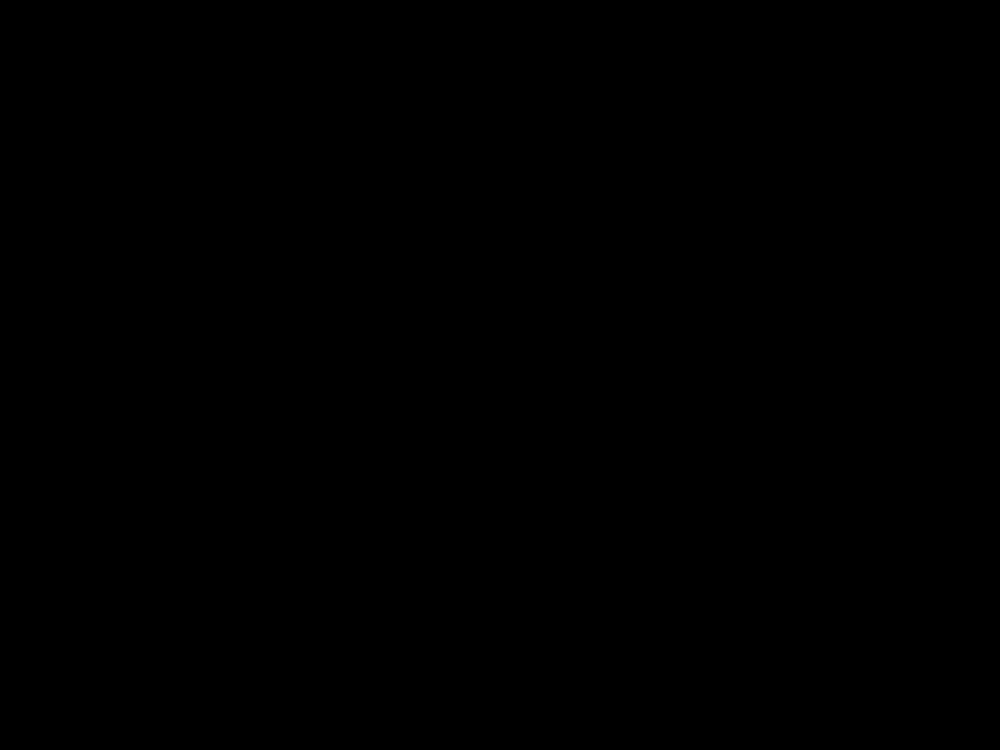
\includegraphics[width=50mm]{images/placeholder.png}}
%   \caption{Description}
% \end{figure}
%-----------------------------------------------

\begin{document}

\setcounter{section}{12}

\section{Lecture 13 (23/03/2020)}
\subsection{Vibrations and oscilations part 2}
Lecture 13 doesn't cover a whole lot of new material since the lectures covered chapter 22 earlier on (Lecture 05). It does have a little new material in the form of a problem involving rotations but these lecture notes will mainly just be example problems.

\subsection{Ideal springs vs non-ideal springs}
Before the example there will be a short subsection clearing up confusion between springs with a zero-length and ideal springs.\\
An ideal spring is a spring where for any elongation it will exert a spring force $F_v = ks$. This is illustrated in the figures below.
\begin{figure}[h]
  \centering
  \subfloat[$y=0$]{{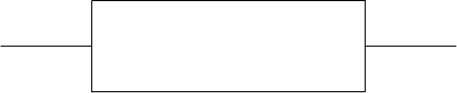
\includegraphics[width=30mm]{images/Ideal_Spring_a.png}}}%
  \qquad
  \subfloat[$y$ is positive]{{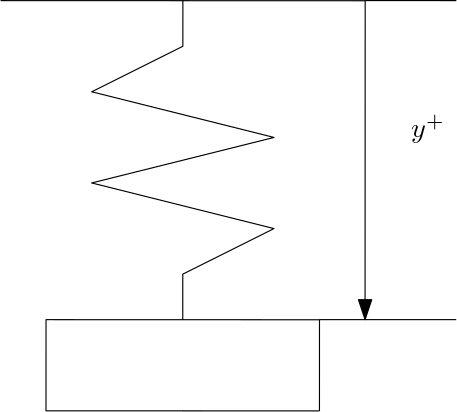
\includegraphics[width=30mm]{images/Ideal_Spring_b.png}}}%
  \qquad
  \subfloat[$y$ is negative]{{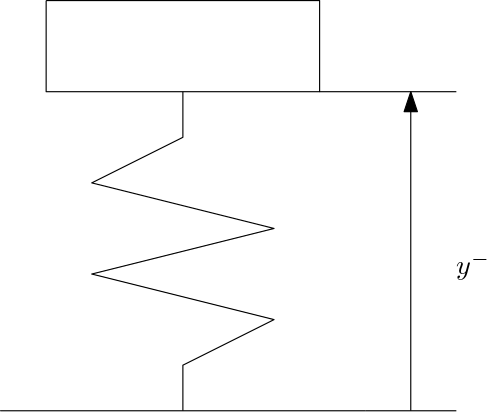
\includegraphics[width=30mm]{images/Ideal_Spring_c.png}}}
  \caption{Force from an ideal spring}
\end{figure}
Ideal springs are good for math since they're easy to work with but not so good for realistic results, since ideal springs don't actually exist. In general a real spring will have a zero-length, which is the length in which the spring exerts exactly no force. The principal of a spring with a zero-length is shown in the figure below.
\begin{figure}[h]
  \centering
  \subfloat[$y=0$]{{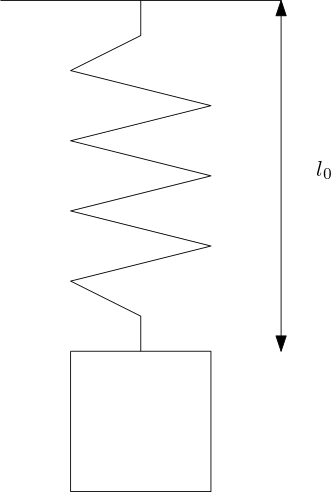
\includegraphics[width=30mm]{images/Non_ideal_spring_a.png}}}%
  \qquad
  \subfloat[Datum at $l_0$]{{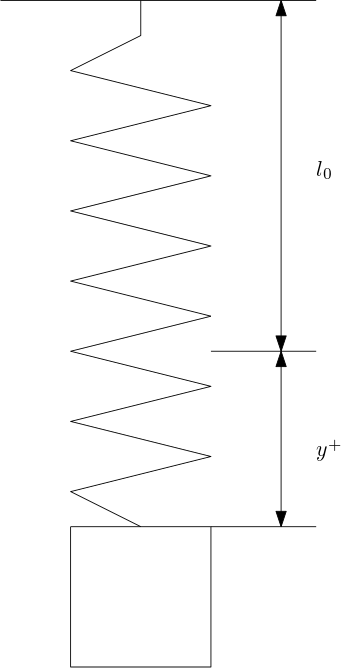
\includegraphics[width=30mm]{images/Non_ideal_spring_b.png}}}%
  \qquad
  \subfloat[Datum at $0$]{{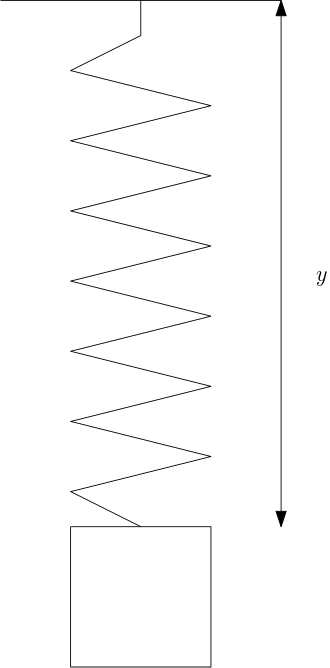
\includegraphics[width=30mm]{images/Non_ideal_spring_c.png}}}
  \caption{Force from a non-ideal spring}
\end{figure}

\subsection{Spring with damper}
\setcounter{equation}{0}
Templates for images and figures
\begin{figure}[h]
  \centering
  \subfloat[Situation]{{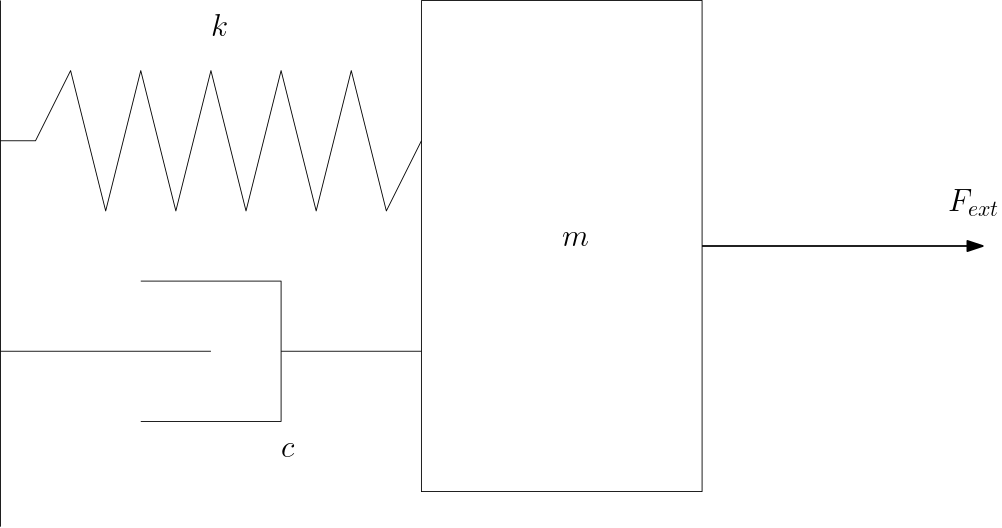
\includegraphics[width=50mm]{images/Spring_with_damper_situation.png}}}%
  \qquad
  \subfloat[FBD]{{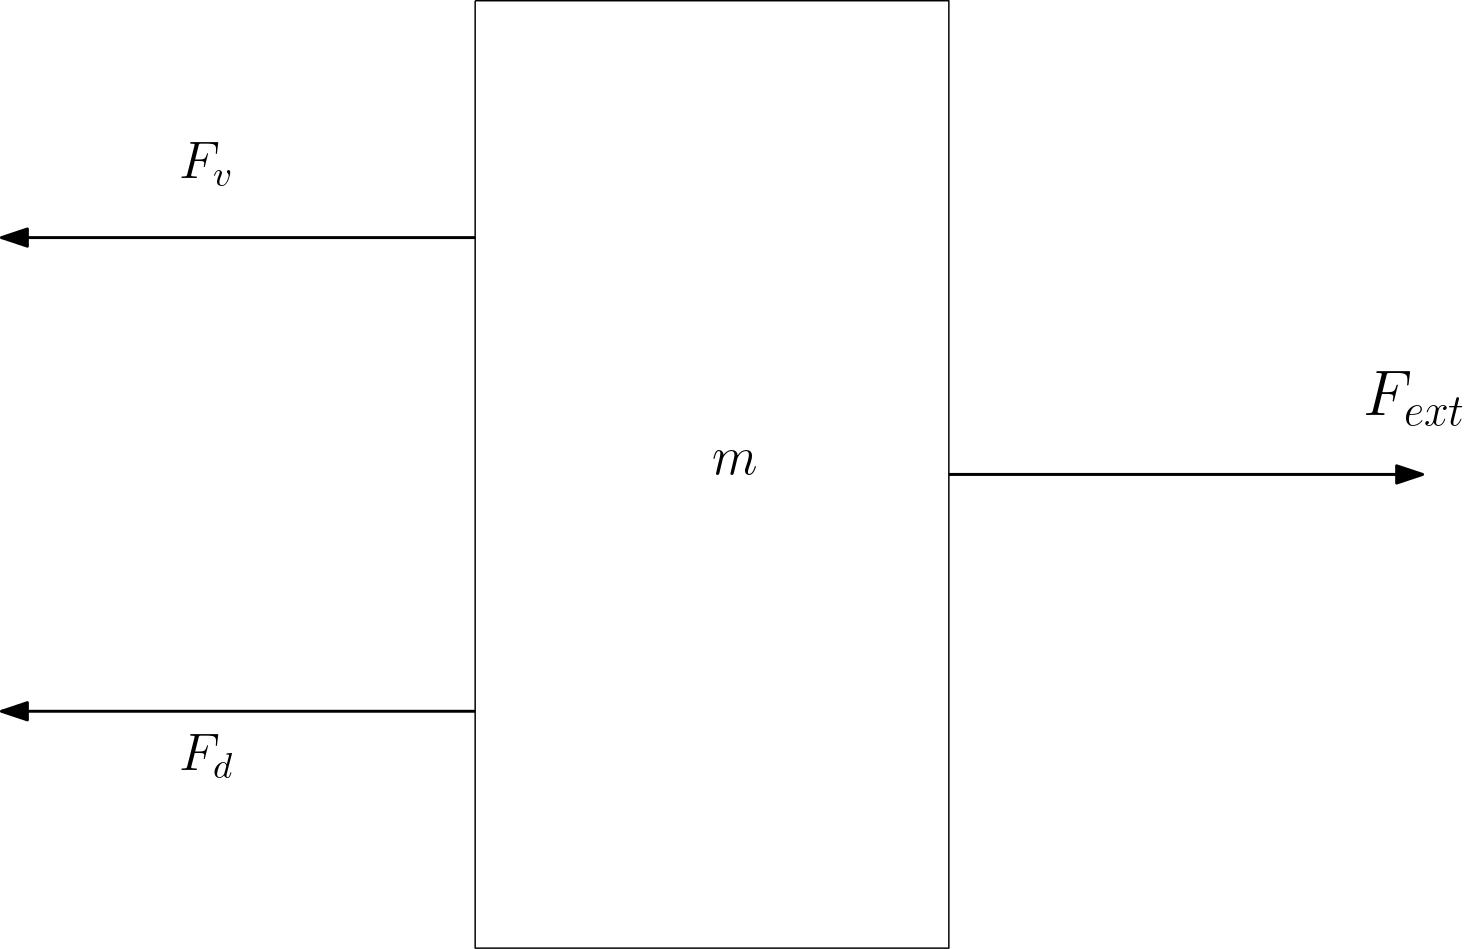
\includegraphics[width=50mm]{images/Spring_with_damper_FBD.png}}}%
  \caption{Oscilating spring with damper term}
\end{figure}
\begin{gather}
  \Sigma F_x = F_{ext} - F_v - F_d = m\ddot{x}\\
  F_v = kx\\
  F_d = c\dot{x}
\end{gather}
Subsitute equations (2) and (3) into (1):
\begin{gather}
  F_{ext} - kx - c\dot{x} = m\ddot{x} \notag \\
  m\ddot{x} + c\dot{x} + kx = F_{ext}
\end{gather}
Where equation (4) is a non-homogeneous 2nd order linear ODE\footnote{Ordinary differential equation}.

\subsection{Rotating oscilation problem with Torsion rod}
\setcounter{equation}{0}
\begin{figure}[h]
  \centering
  \subfloat[Situation]{{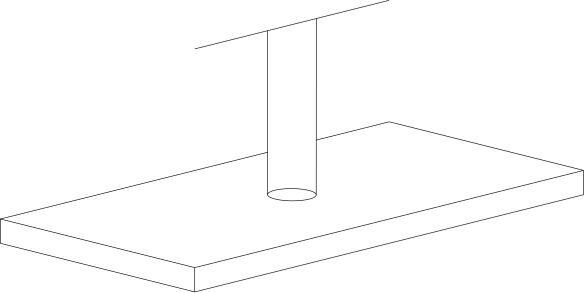
\includegraphics[width=50mm]{images/Torsion_rod_situation.png}}}%
  \qquad
  \subfloat[FBD]{{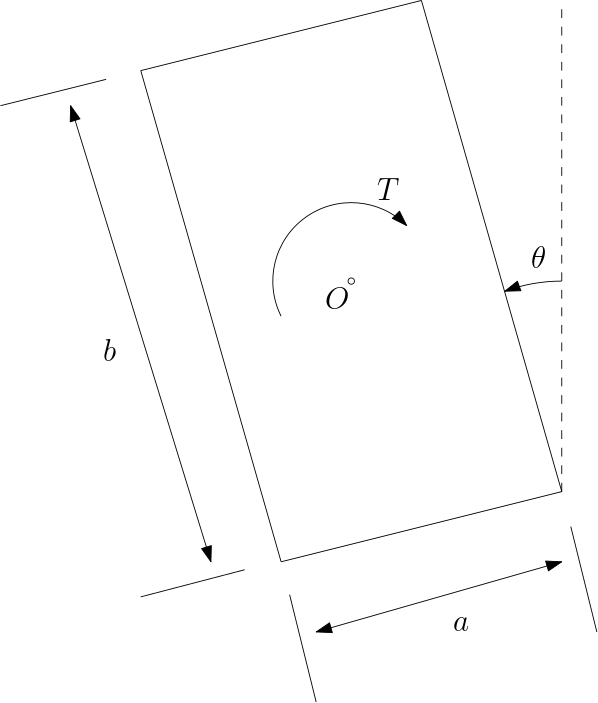
\includegraphics[width=50mm]{images/Torsion_rod_FBD.png}}}%
  \caption{Oscilating plate on a torsion rod}
\end{figure}
\begin{gather}
  \Sigma M_O = -T = I_O\ddot{\theta}\\
  T = k\theta\\
  I_O = \frac{1}{12}m(a^2 + b^2)
\end{gather}
Subsitute equation (2) and (3) into (1):
\begin{gather}
  -k\theta = \frac{1}{12}m(a^2 + b^2)\ddot{\theta} \notag \\
  \frac{1}{12}m(a^2 + b^2)\ddot{\theta} + k\theta = 0
\end{gather}
Where (4) is the homogeneous 2nd order linear ODE.

\subsection{Complex spring systems example}
\setcounter{equation}{0}
There will be situation where computations will be done for spring systems where the oscilation will not be one single spring vibrating, but any random combination of springs in a series or parallel. The following example will cover such a system with 2 springs placed in series with eachother.
\begin{figure}[h]
  \centering
  \subfloat[Situation]{{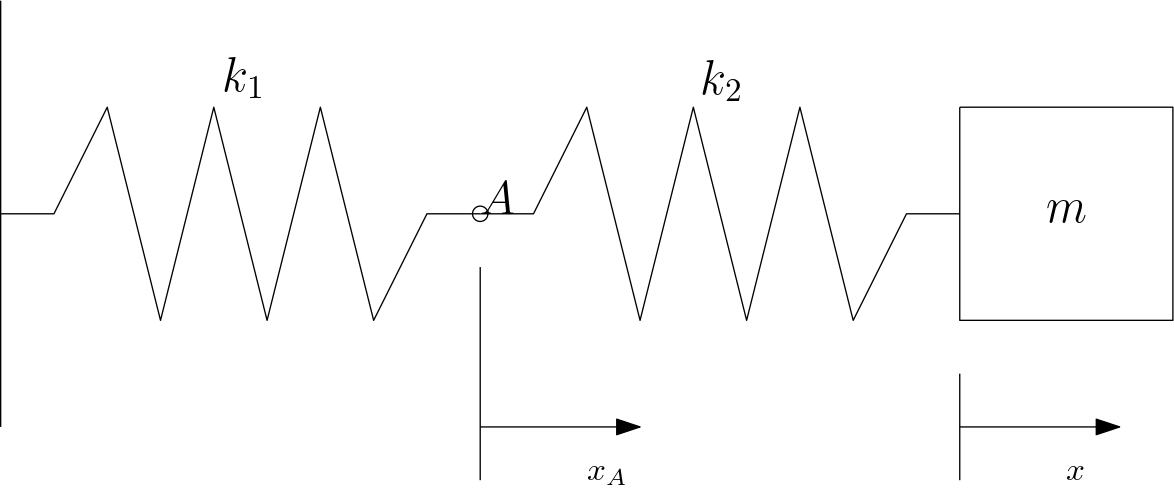
\includegraphics[width=30mm]{images/Series_springs_situation.png}}}%
  \qquad
  \subfloat[FBD springs]{{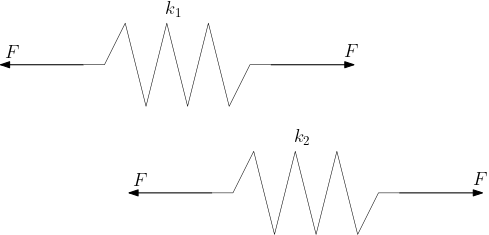
\includegraphics[width=30mm]{images/Series_springs_FBD_1.png}}}%
  \qquad
  \subfloat[FBD mass]{{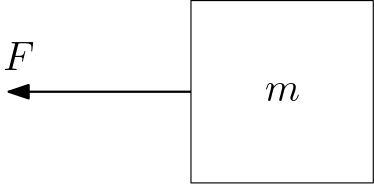
\includegraphics[width=30mm]{images/Series_springs_FBD_2.png}}}%
  \caption{Spring system with springs in series rather then a single oscilating spring}
\end{figure}
Since Newton's 3rd law states Action = -Reaction:
\begin{gather}
  F = k_1x_A \Rightarrow x_A = \frac{F}{k_1} \notag\\
  F = k_2(x-x_A) \Rightarrow F = k_2x - \frac{k_2}{k_1}F \notag\\
  F = \frac{k_1k_2}{k_1 + k_2}x
\end{gather}
Then when considering the FBD of the vibrating mass:
\begin{gather}
  \Sigma F_x = -F = m\ddot{x} \notag\\
  -\frac{k_1k_2}{k_1 + k_2}x = m\ddot{x} \notag\\
  m\ddot{x} + \frac{k_1k_2}{k_1 + k_2}x = 0
\end{gather}
Where $m\ddot{x} + \frac{k_1k_2}{k_1 + k_2}x = 0$ would be the homogeneous Linear 2nd order ODE that needs to be solved for the answer.

\subsection{Example with non-ideal spring and gravity}
\setcounter{equation}{0}
\begin{figure}[h]
  \centering
  \subfloat[Situation]{{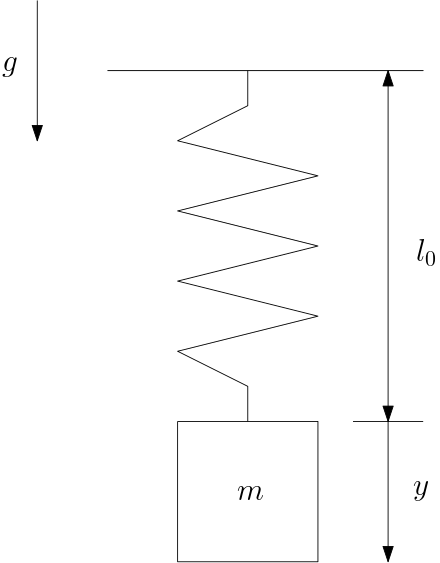
\includegraphics[width=30mm]{images/Non_ideal_spring_Situation.png}}}%
  \qquad
  \subfloat[FBD]{{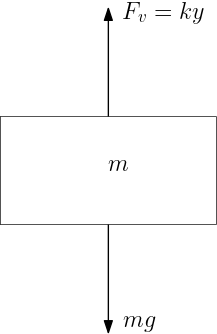
\includegraphics[width=30mm]{images/Non_ideal_spring_FBD.png}}}%
  \caption{Oscilating non-ideal spring with gravity term}
\end{figure}
\begin{gather}
  \Sigma F_y = mg - ky = m\ddot{y}\\
  \text{Equilibrium when $\ddot{y} = 0$} \notag \\
  mg - ky = 0 \notag \\
  y = y_e = \frac{mg}{k}\\
  \text{where $y_e$ is the equilibrium position} \notag
\end{gather}
\begin{gather}
  m\ddot{y} + ky = mg
\end{gather}
Equation (3) is a non-homogenous 2nd order linear ODE. The solution to this type of differential equation will take the form of $y = y_p + y_c$ where $y_p$ is the particular solution and $y_c$ is the characteristic equation. The particular solution is found by "geussing" the solution takes the same for as the right hand side of the equation. In this case this means that the solution is of the form $y_p = C$, where $C$ is some constant. This gives the following:
\begin{align}
  \begin{cases}
    y_p = C\\ 
    y'_p = 0\\
    y''_p = 0\\
  \end{cases}
  \Rightarrow
  m \cdot 0 + kC &= mg\\
  C &= \frac{mg}{k} = y_p
\end{align}
For the characteristic eqution we guess the solution is of the form $y_c = e^{\lambda y}$. This gives the following:
\begin{align}
  \begin{cases}
    y = e^{\lambda y}\\
    y' = \lambda e^{\lambda y}\\
    y'' = \lambda^2 e^{\lambda y} 
  \end{cases}
  \Rightarrow
  m\lambda^2 e^{\lambda y} + k\lambda e^{\lambda y} = 0\\
  e^{\lambda y} \neq 0,\; \text{Thus:} \notag\\ 
  m\lambda^2 + k\lambda = 0 \notag\\
  \lambda(m\lambda + k) = 0 \notag\\
  \lambda_1 = 0 \wedge \lambda_2 = -\frac{k}{m}\\
\end{align}
The total characteristic solution then becomes:
\begin{align}
  y_c &= C_1e^{\lambda_1 y} + C_2e^{\lambda_2 y}\\
      &= C_1 + C_2e^{-\frac{k}{m}y}
\end{align}
Where $C_1$ and $C_2$ are random constants which can be determined by solving for the initial conditions of the problem. The total solution for ht edifferential equation then becomes:
\begin{equation}
  y = y_p + y_c = \frac{mg}{k} + C_1 + C_2e^{-\frac{k}{m}y}
\end{equation}
\end{document}